%-----------------------------------------------------------------
%	ESCALA DE MAGNITUDS ESTEL·LARS
%	!TEX root = ./../main.tex
%-----------------------------------------------------------------
\section{Escala de magnituds estel·lars}
\subsection{Escala de magnituds estel·lars}
% FIXME: hipparcus@sec:bio
Hiparc de Rodes ($\approx$ 190--120 aC) va assignar magnitud aparent $m = 1$ a l'estrella més brillant del firmament i, descendent, $m=6$ a la menys brillant (a simple vista).

\subsubsection*{Fotòmetre}
És un instrument ideat per mesurar la brillantor d'una estrella. Quan la llum d'aquesta incideix sobre una superfície foto-sensible es crea un corrent per efecte fotoelèctric. La llum rebuda al telescopi passa, a través d'un filtre, a una superfície sensible a la llum coneguda com a càtode. El càtode emet electrons que són multiplicats per un foto-multiplicador, de tal manera que el senyal és fàcilment mesurable. Cada fotó detectat pel càtode genera un pols; el nombre de polsos per segon és proporcional a la brillantor de l'estrella. En fotometria d'alta velocitat els polsos són comptats en intervals molt més curts que 1 segon. Hi fotòmetres capaços de mesurar magnituds estel·lars amb un error màxim proper a la mil·lèsima de magnitud $m$.

\begin{defi}[Lluminositat, $L$]
	Energia emesa per una estrella per unitat de temps. Al CGS té unitats de $\qty[L] = \si{\erg\per\s}$.
\end{defi}

\begin{defi}[Flux radiant, $F$]
	Assumint que la llum no és absorbida durant el seu viatge al fotòmetre, el flux radiant mesurat a una distància $r$ està relacionat amb la lluminositat $L$ de l'estrella per
	\begin{align}
		F = \frac{L}{4\pi r^{2}}
	\end{align}
	que és l'energia rebuda per unitat d'àrea i de temps ($\si{\erg\per\square\cm\per\s}$).
\end{defi}

\begin{example}
	La lluminositat del Sol és $\Lsun = \SI{3.826 e33}{\erg \per \s}$, a la distància de $\SI{1}{\au} = \SI{1.496 e13}{\cm}$. Llavors, la Terra rep un flux radiant just per sobre de la seva atmosfera (que és absorbent):
	\begin{align*}
		F_{\odot} = \frac{\num{3.826 e33}}{4\pi (\num{1.496 e13})^{2}} = \SI{1.360 e6}{\erg \per \square\cm \per \s}
	\end{align*}
	Aquest valor s'anomena \textit{constant solar}.
\end{example}

\begin{defi}[Magnitud aparent, $m$]
	Siguin $F_{1}$ i $F_{2}$ els fluxos radiants rebuts de dues estrelles (suposant que no hi ha absorció), llavors la diferència en magnituds aparents es defineix com
	\begin{align}
		m_{1} - m_{2} = -2.5 \log(\frac{F_{1}}{F_{2}}) % \Leftrightarrow \frac{F_{2}}{F_{1}} = 100^{(m_{1}-m_{2})/5}
	\end{align}
	o bé
	\begin{align}
		\frac{F_{2}}{F_{1}} = 100^{(m_{1}-m_{2})/5}
	\end{align}
	La magnitud aparent $m$ depèn de $L$ i de $r$.
\end{defi}

\begin{defi}[Magnitud absoluta, $M$]
	És la magnitud aparent que tindria una estrella si estigués a $\SI{10}{\parsec}$ de nosaltres.
	\begin{align}
		100^{(m - M)/5} = \frac{F_{10}}{F} = \qty(\frac{d}{\SI{10}{\parsec}})^{2} \Rightarrow d = 10^{(m - M + 5)/5} \si{\parsec}
	\end{align}
\end{defi}

\begin{defi}[Distància mòdul, $\mu = m - M$]
	Dóna una indicació de la distància $d$ en què es troba una estrella de la Terra.
	\begin{align}
		m - M = 5 \log(\frac{d}{\SI{10}{\parsec}})
	\end{align}
\end{defi}

% \begin{example}
%     Sabent que la magnitud aparent del Sol (a $\SI{1}{\au}$ de la Terra) és $m_{\odot} = -26.81$, trobeu la seva magnitud absoluta.
%     \begin{align*}
%         \Msun & = m_{\odot} - 5 \log(\frac{d}{\SI{10}{\parsec}}) = 4.76
%     \end{align*}
% \end{example}

\begin{example}
	La magnitud absoluta d'una estrella a la Galàxia Andròmeda (a \SI{690}{\kilo \parsec} de nosaltres) és $M = 5$. L'estrella explota sobtadament donant lloc a una supernova de magnitud aparent $m = 6.7$. Trobeu: (a) el quocient entre les lluminositats intrínseques de la supernova, $L_{2}$, i l'estrella progenitora, $L_{1}$; (b) La magnitud absoluta de la supernova.
	\begin{Lalign}\tag{a}
	\begin{gathered}
		d = 10^{(m-M+5)/5} \si{\parsec} \Rightarrow m_{1} = -5 + M_{1} + 5 \log d = 29.19 \\
		m_{1} - m_{2} = -2.5 \log(\frac{F_{1}}{F_{1}}) \Rightarrow \log(\frac{L_{2}}{L_{1}}) = \frac{m_{1}-m_{2}}{2.5} = 8.99\\
		\Rightarrow \frac{L_{2}}{L_{1}} = 10^{8.99} \approx \num{9.9 e8}
	\end{gathered}
	\end{Lalign}
	\begin{Lalign}\tag{b}
		d &= 10^{(m-M+5)/5} \si{\parsec} \Rightarrow M_{2} = m_{2} + 5 - 5 \log d = -17.49
	\end{Lalign}
\end{example}

\begin{example}
	La magnitud aparent d'una sistema estel·lar triple és $m = 0.0$. Dues de les seves components posseeixen magnituds $m_{A} = 1.0$ i $m_{B} = 2.0$. Quina és la magnitud de la tercera component?
	\begin{align*}
		m - m_{0} = -2.5 \log(\frac{F}{F_{0}})
	\end{align*}
	Triem $m_{0} = 0$ (és a dir, $F_{0} = 1$), llavors
	\begin{align*}
		m = -2.5 \log F
	\end{align*}
	Trivialment trobem $F_{A}$ i $F_{B}$. Per una altra part, tenim que
	\begin{align*}
		m_{total} = -2.5 \log F_{total} = -2.5 \log (F_{A} + F_{B} + F_{C})
	\end{align*}
	Llavors,
	\begin{align*}
		m_{C} = -2.5 \log[F_{total} - (F_{A} + F_{B})] = 0.89
	\end{align*}
\end{example}

Si dues estrelles $A$ i $B$ es troben a la mateixa distància de la Terra, tindrem
\begin{align*}
	100^{(M_{A}-M_{B})/5} = \frac{L_{B}}{L_{A}}
\end{align*}
i si una de elles és el Sol, la magnitud absoluta de l'altra estrella serà
\begin{align}
	M = \Msun - 2.5 \log(\frac{F}{F_{10,\odot}})
\end{align}

Fins aquí hem considerat magnituds bolomètriques (totes les longituds de l'espectre visible) i hem menyspreat l'extinció i l'absorció. En general, es compleix
\begin{align}
	m_{\lambda} - M_{\lambda} = 5 \log(\frac{d}{\SI{10}{\parsec}}) + a_{\lambda}
\end{align}
on $a_{\lambda}$ és un factor de correcció que té en compte l'absorció a la longitud d'ona $\lambda$.

%-----------------------------------------------------------------
\subsection{Determinació de distàncies astronòmiques}
\subsubsection*{Polsos de radar}
\begin{figure}[H]
	\centering
	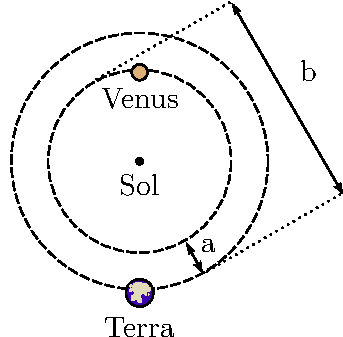
\includegraphics[width=0.3\textwidth]{./images/2-radar-venus-earth}
	\caption{Diagrama il·lustratiu del sistema Terra--Venus i les seves òrbites al voltant del Sol}
	\label{fig:radar}
\end{figure}

Mitjançant polsos de radar s'ha aconseguit trobar la distància a Venus\footnote{El semieix major de l'òrbita de Venus respecte el Sol és $\approx \SI{0.7233}{\au}$.} amb $\SI{\pm 1}{\km}$ de precisió. Un cop coneguda la distància a Venus quan està més a prop de la Terra, $a$, i quan està més lluny, $b$, es veu trivialment que la distància al Sol és
\begin{align*}
	d(\oplus, \odot) = \frac{a+b}{2} \equiv \SI{1}{\au} \approx \SI{1.496 e13}{\cm}
\end{align*}

\subsubsection*{Paral·laxi trigonomètrica}
És un mètode que s'utilitza per mesurar la distància a una estrella \textit{propera}. L'estrella és observada des d'extrems oposats de l'òrbita terrestre (6 mesos entre dues observacions successives) respecte el fons \textit{immòbil} d'estrelles.
\begin{figure}[ht]
	\centering
	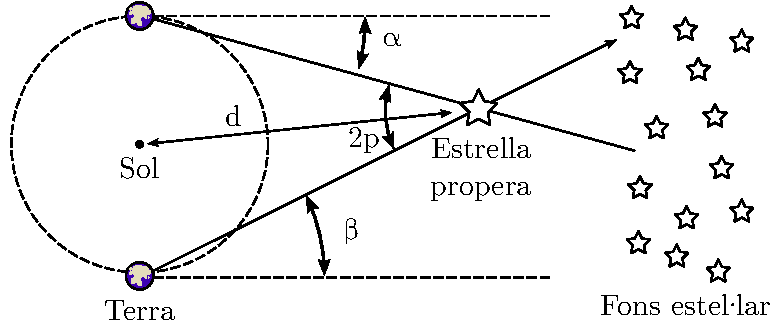
\includegraphics[width=0.7\textwidth]{./images/2-trig-parallax}
	\caption{Diagrama de l'observació de la posició relativa d'una estrella propera respecte el fons d'estrelles llunyanes}
	\label{fig:trig-parallax}
\end{figure}

\begin{align}
	p = \frac{1}{2} (\alpha + \beta) \Rightarrow d = \frac{1}{p\si{\arcsecond}}
\end{align}
Una estrella de paral·laxi $p = \SI{1}{\arcsecond}$ es troba a $\SI{1}{\parsec} \approx \SI{2.063 e5}{\au}$ (parsec) de distància de la Terra.

El satèl·lit \textit{Hipparcos} ha obtingut posicions de més de 120 mil estrelles amb gran precisió ($\sim \SI{e-3}{\arcsecond}$) fins a distàncies de $\SI{100}{\parsec}$ (això dota una precisió del $\SI{10}{\percent}$ a aquesta distància).

\subsubsection*{Paral·laxi espectroscòpica}
És un mètode que fa ús de les línies espectrals. Un cop coneguda la distància a les estrelles pròximes, es pot relacionar la seva brillantor absoluta, o lluminositat, amb el seu tipus espectral.

Astronòmicament les estrelles més brillants de cada tipus espectral es converteixen en indicadors de distància a distàncies tals que només les estrelles més brillants poden ser observades individualment (a tals distàncies la paral·laxi trigonomètrica ja no és útil).

\subsubsection*{Mètode del cúmul en moviment}
És un mètode vàlid per determinar la distància a un cúmul estel·lar (de mida $D \ll d$) els membres del qual són pròxims i es desplacen en grup.
\begin{figure}[ht]
	\centering
	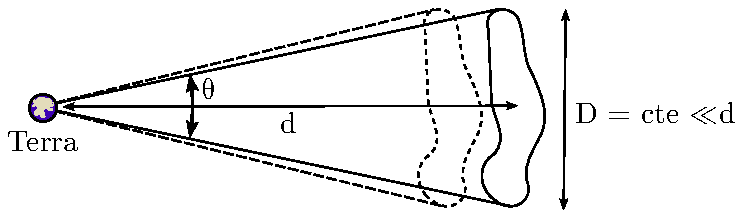
\includegraphics[width=0.7\textwidth]{./images/2-cluster-mov}
	\caption{Diagrama de l'observació d'un cúmul en moviment per determinar la seva distància}
	\label{fig:cluster-mov}
\end{figure}

\begin{align}
	\theta = \frac{D}{d} \Rightarrow \dot{\theta} = - D\frac{d}{d^{2}} \Rightarrow d = - v \frac{\theta}{\dot{\theta}}
\end{align}
La  velocitat $v$ del cúmul al llarg de la visual ve donada pel desplaçament Doppler de les línies espectrals; $\dot{\theta}$ es determina comparant la posició de les estrelles en plaques fotogràfiques preses amb desenes d'anys de diferència.

Aquest mètode només s'ha emprat amb èxit en la determinació de la distància al Cúmul de les Híades ($ \approx \SI{48}{\parsec}$).

\subsubsection*{Superposició de seqüències principals}
Es basa en la hipòtesi que les estrelles de la seqüència principal\footnote{A la pàgina \pageref{sec:hertz-russell} es fa un tractament més profund dels diagrames de Hertzsprung--Russell i el significat de la seqüència principal.} tenen idèntiques propietats amb independència del cúmul al qual pertanyen. Llavors, el pendent de la seqüència principal serà el mateix en tots els cúmuls i les estrelles de la seqüència principal del mateix tipus espectral o color tenen la mateixa magnitud absoluta independentment del cúmul.

Sota aquesta hipòtesi, podem comparar la lluminositat de les estrelles en la seqüència principal del Cúmul de les Híades amb les de qualsevol altre cúmul.

El desplaçament vertical per superposar ambdós cúmuls dóna la distància relativa entre ambdós cúmuls:
\begin{align}
	\Delta m \equiv m_{GC} - m_{Hya} = 5 \log(\frac{d_{GC}}{d_{Hya}}) + a'
\end{align}
on $a'$ és la correcció deguda a la diferència en l'enrogiment interestel·lar entre ambdós cúmuls; aquesta pot ser determinada per l'ús de les línies espectrals.

\subsubsection*{Estrelles RR Lyrae}
Un cert tipus d'estrelles grogues, gegants, polsants amb període d'oscil·lació entre 0.2 i 1.2 dies, i amb $0.2 \leq \Delta m \leq 2$ magnituds, són de la població II\footnote{Les estrelles de la població I contenen quantitats significatives d'elements més pesats que l'heli (anomenats genèricament \textit{metalls} en astrofísica). Aquests elements foren produïts per generacions anteriors d'estrelles a través d'explosions de supernova. El nostre Sol pertany al grup de població I. Són habituals als braços espirals de la Via Làctia. Les estrelles de la població II són les primeres estrelles de vida llarga formades després del Big Bang i, per tant, contenen poca quantitat de metalls. Es troben en cúmuls globulars i al centre de la Via Làctia. Evidentment, són estrelles molt més velles que les de la població I.} i es troben en l'halo de la galàxia i en cúmuls globulars.

La magnitud aparent, $m$, de totes les RR Lyrae variables resulta ser la mateixa en un cúmul donat (tot i que varia d'un cúmul a un altre), independentment del seu període. Ja que són intrínsecament lluminoses i el seu període les fa destacar, són indicadores ideals de distàncies.

Suposem que la magnitud absoluta, $M$, és la mateixa amb independència del cúmul. Així, la distància entre dos cúmuls pot determinar-se mitjançant la fórmula
\begin{align}
	\Delta m \equiv m_{1} - m_{2} = 5 \log(\frac{d_{1}}{d_{2}}) + a'
\end{align}

\subsubsection*{Estrelles variables Cefeides}
% FIXME: leavitt@sec:bio
Estrelles grogues, gegants o supergegants, de lluminositat variable observades per primer cop als Núvols de Magalhães (galàxies nanes del nostre Grup Local). La seva importància deriva de la relació (descoberta per Henrietta Leavitt) entre període i magnitud absoluta (al visible).
\begin{align}\label{eq:cepheid}
	M_{v} = (-2.43 \pm 0.12) (\log(T) - 1) - (4.05 \pm 0.02)
\end{align}
Llavors, observant el període coneixem la magnitud absoluta $M$, i mitjançant l'expressió
\begin{align}
	M = \Msun - 2.5 \log(\frac{L}{\Lsun})
\end{align}
determinem la seva lluminositat $L$. Coneguda $L$ i el seu flux lumínic que arriba a la Terra es troba la distància.
\begin{figure}[h]
	\centering
	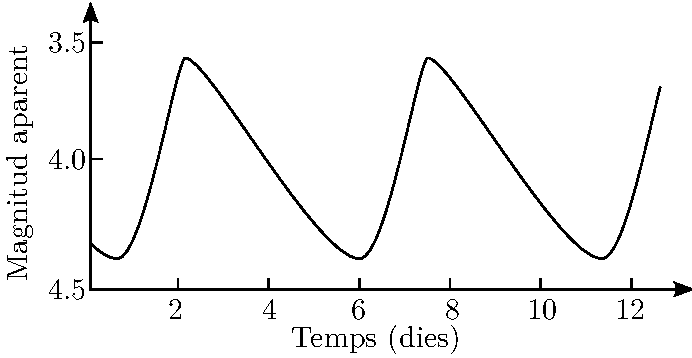
\includegraphics[width=0.6\textwidth]{./images/2-cepheid}
	\caption{Corba de llum de la Cefeida $\delta$--Cephei, amb magnitud variable $m$ (entre $\numrange{3.6}{4.3}$) en un període de 5.4 dies}
	\label{fig:cepheid}
\end{figure}

\subsubsection*{Noves}
La seva magnitud absoluta, $M$, està relacionada amb el ritme de decreixement de lluminositat després d'un \textit{outburst}. L'enorme lluminositat intrínseca d'una nova fa d'ella un indicador molt útil de distàncies en el cas de galàxies properes.

\subsubsection*{Supernoves}
S'han observat explosions de supernoves fins a distàncies corresponents a \textit{redshift} $z = 2$. La lluminositat de les supernoves pot determinar-se si es coneix (a través de l'observació) el ritme de decreixement de la seva lluminositat. Tanmateix, observacions a diferents longituds d'ona permeten calibrar l'extinció ocasionada per la pols interestel·lar, que podria conduir a una falsa estimació de la distància.

El primer registre d'una supernova és la Supernova Tycho (una de les vuit supernoves que han estat visibles a simple vista), observada pel famós astrònom Tycho Brahe l'11 de novembre de 1572 [\href{http://apod.nasa.gov/apod/ap990307.html}{APOD~990307}].

\subsubsection*{Relació Tully--Fisher}
Relació empírica entre l'amplada de la línia de $\SI{21}{\cm}$ de l'hidrogen neutre (\textit{spin-flip} d'electró--protó, $\Delta E = hc/\lambda = \SI{6 e-6}{\eV}$) a galàxies espirals (causada per la seva rotació) i la lluminositat:
\begin{align}
	\frac{L_{H}}{\num{3 e10} L_{H\odot}} \approx \qty[\frac{v_{\max}}{\SI{196}{\km\per\s}}]^{3.8}
\end{align}
Aquesta relació es pot utilitzar per determinar la distància relativa entre galàxies espirals així com entre grups de galàxies.

Ja que la matèria fosca contribueix notablement a $v_{\max}$ però no contribueix a la lluminositat, aquesta relació empírica és difícil d'entendre.

\subsubsection*{Relació entre la distància i els desplaçament cap al roig}
Observant els objectes més brillants de les galàxies (tals com estrelles O, noves, Cefeides variables, les quals poden ser detectades fins i tot en les galàxies més properes del Cúmul de Virgo) s'adverteix la relació empírica $z \propto d$, on $z$ es defineix com
\begin{align}
	z = \frac{\Delta \lambda}{\lambda} = \frac{\lambda_{obs} - \lambda_{em}}{\lambda_{em}}
\end{align}

Així, si una galàxia és observada a \textit{redshift} $z_{1}$ i una altra a $z_{2}$, la relació de distàncies entre elles serà
\begin{align}
	\frac{d_{1}}{d_{2}} = \frac{z_{1}}{z_{2}}
\end{align}
\begin{figure}[H]
	\centering
	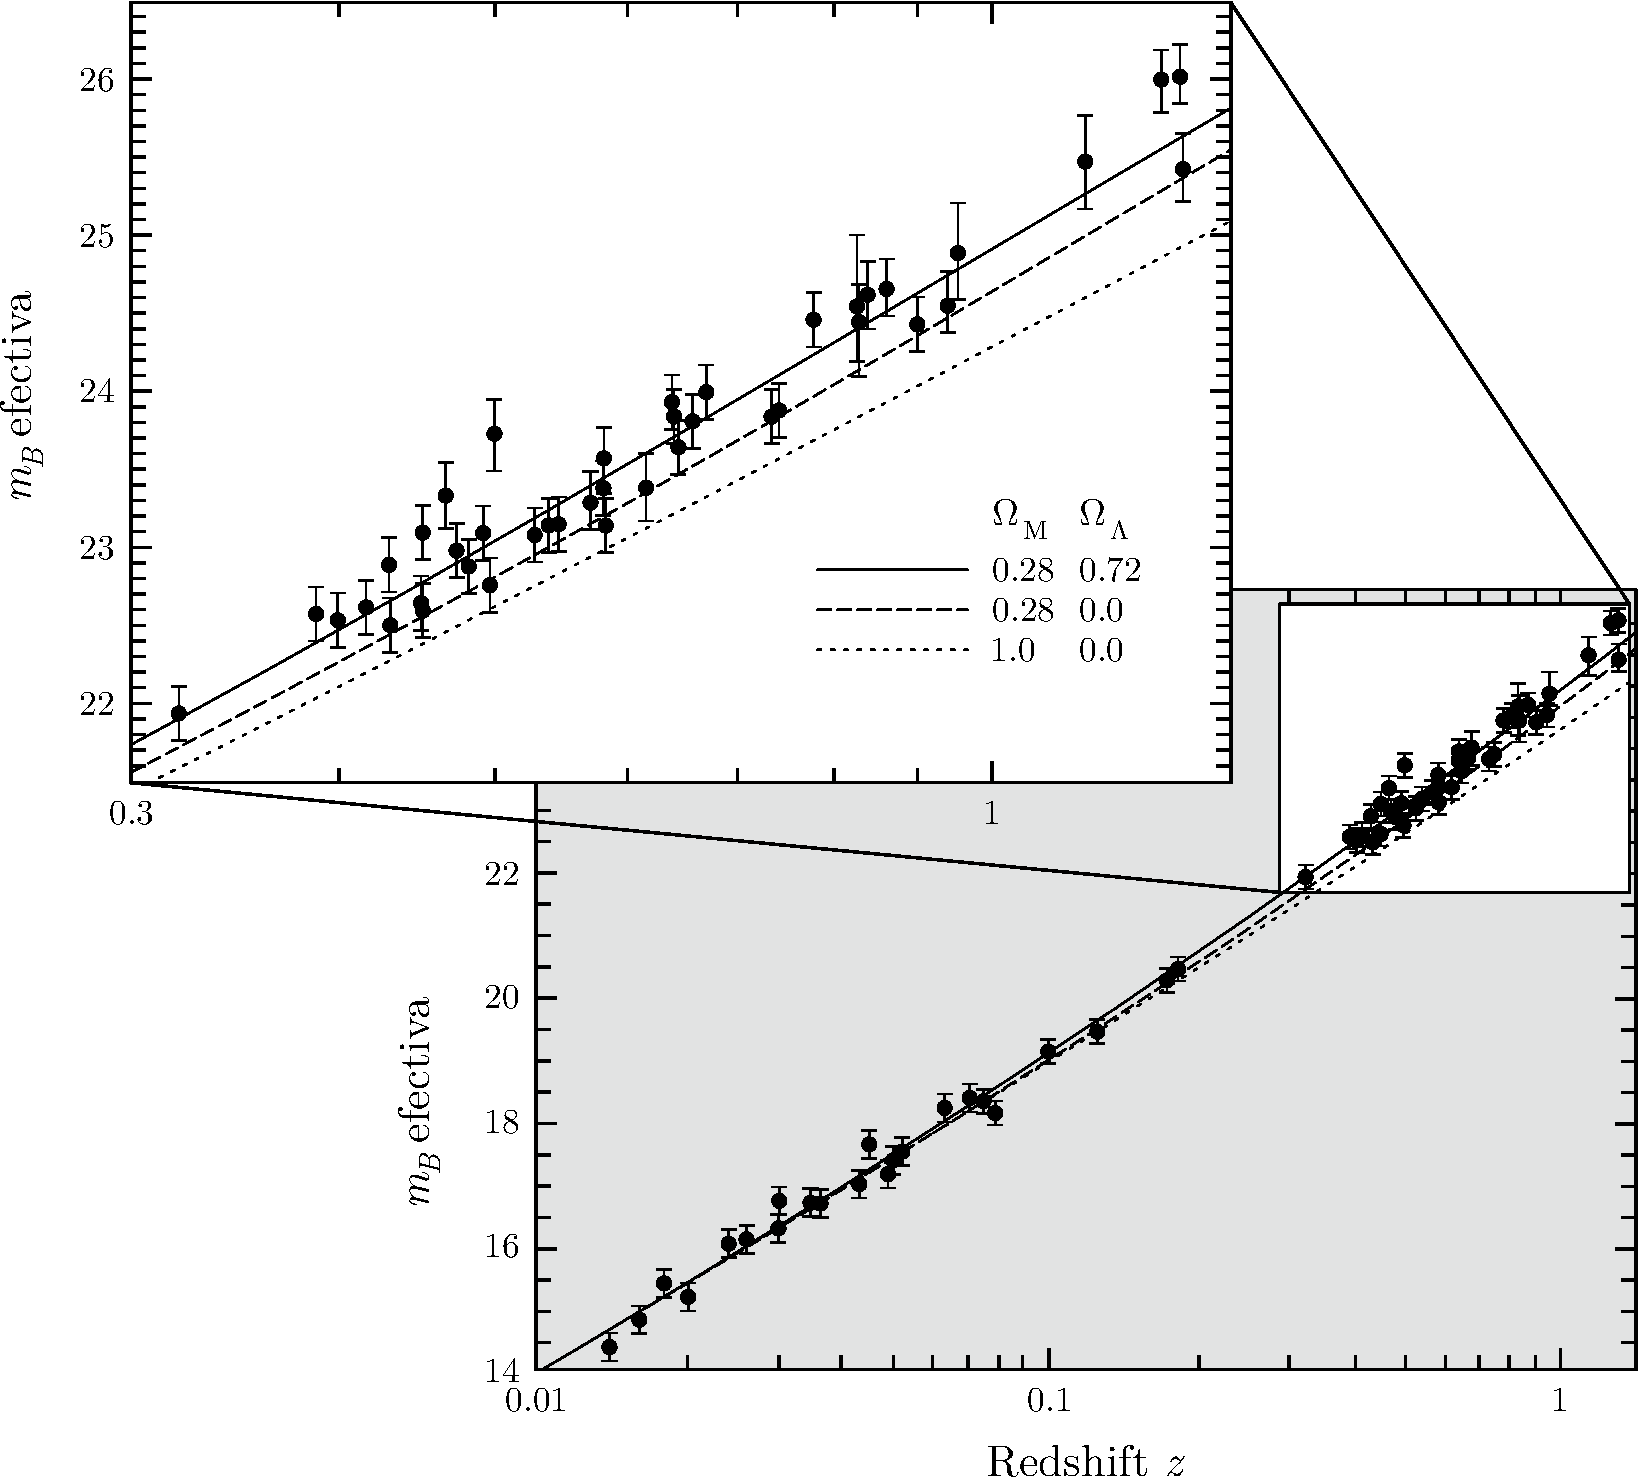
\includegraphics[width=0.9\textwidth]{./images/2-supernovae-redshift}
	\caption{Magnitud efectiva en el blau de supernoves en funció del \textit{redshift}}
	\label{fig:supernovae-redshift}
\end{figure}

És important, no obstant això, utilitzar galàxies del mateix tipus (podeu trobar la classificació dels tipus de galàxies a la \S~\ref{sec:galaxies}).

%-----------------------------------------------------------------
\subsection{Índex de color}
A la magnitud aparent, $m$, i l'absoluta, $M$, preses sobre totes les longituds d'ona de la llum emesa per una estrella se les anomena \textit{magnituds bolomètriques}, $m_{bol}$ i $M_{bol}$, respectivament.

Però, en realitat, la majoria de detectors mesuren el flux lluminós d'una estrella només dins d'algun interval $\Delta \lambda$ que depèn de la sensibilitat del detector.

El color d'una estrella pot determinar-se amb certa precisió mitjançant filtres que permeten el pas de la llum només en un rang donat de longituds d'ona.

En el sistema estàndard U, B, V, la magnitud aparent d'una estrella es mesura a través de tres filtres:
\begin{itemize}
	\item U: magnitud ultraviolada de l'estrella, es mesura amb un filtre centrat en $\SI{3650}{\angstrom}$ amb una amplada de $\SI{680}{\angstrom}$.
	\item B: magnitud blava de l'estrella, es mesura amb un filtre centrat en $\SI{4400}{\angstrom}$ amb una amplada de $\SI{980}{\angstrom}$.
	\item V: magnitud visual de l'estrella, es mesura amb un filtre centrat en $\SI{5500}{\angstrom}$ amb una amplada de $\SI{890}{\angstrom}$.
\end{itemize}

Si es coneix la distància $d$ a l'estrella un cop mesurades $U$, $B$, i $V$, mitjançant l'equació \eqref{eq:mMcolour} es poden determinar les magnituds absolutes de color $M_{U}$, $M_{B}$, i $M_{V}$:
\begin{align}\label{eq:mMcolour}
	m - M = 5 \log(\frac{d}{\SI{10}{\parsec}})
\end{align}

L'\textit{índex de color} $(U-B)$ d'una estrella és la diferència entre les seves magnituds ultraviolada i blava. De forma similar, l'índex de color $(B-V)$ d'una estrella és la diferència entre la magnitud blava i la visual, és a dir,
\begin{align}
\begin{aligned}
	U - B &= M_{U} - M_{B} \\
	B - V &= M_{B} - M_{V}
\end{aligned}
\end{align}
En vista de l'equació \eqref{eq:mMcolour}, l'índex de color no depèn de la distància a l'estrella.

Com que les magnituds decreixen amb la lluminositat, una estrella amb menor índex de color $(B-V)$ és \textit{més blava} que una amb major $(B-V)$.

Finalment, la magnitud bolomètrica, $m_{bol}$, d'una estrella i la seva magnitud visual estan relacionades mitjançant la seva correcció bolomètrica, $BC$, definida com
\begin{align}
	BC = m_{bol} - V = M_{bol} - M_{V}
\end{align}
